\documentclass[12pt]{article}
	
\title{CSC 320 - Worksheet 6}
\author{Nadeem Abdul Hamid}
\date{February 13, 2024}  


\usepackage[margin=1in]{geometry}		% For setting margins
\usepackage{amsmath}				% For Math
\usepackage{amsthm}
\usepackage{fancyhdr}				% For fancy header/footer
\usepackage{graphicx}				% For including figure/image
\usepackage{cancel}					% To use the slash to cancel out stuff in work
\usepackage[shortlabels]{enumitem}
\usepackage{hyperref}
\usepackage{jigsaw}

\usepackage{algorithm,caption}
\usepackage{algpseudocodex}
% docs: https://ctan.math.washington.edu/tex-archive/macros/latex/contrib/algpseudocodex/algpseudocodex.pdf


%%%%%%%%%%%%%%%%%%%%%%
% Set up fancy header/footer
% taken from https://www.overleaf.com/latex/templates/homework-template/yvgnmrbywwnp
\makeatletter    % for \@ in \@title
\pagestyle{fancy}
\fancyhead[LO,L]{\@author}
\fancyhead[CO,C]{\@title}
\fancyhead[RO,R]{\@date}
\fancyfoot[LO,L]{}
\fancyfoot[CO,C]{\thepage}
\fancyfoot[RO,R]{}
\renewcommand{\headrulewidth}{0.4pt}
\renewcommand{\footrulewidth}{0.4pt}
\makeatother    % restore
%%%%%%%%%%%%%%%%%%%%%%


%%%%%%%%%%%%%%%%%%%%%%
% from: https://tex.stackexchange.com/questions/14667/does-latex-define-a-semantic-equivalent-of-textbf
\makeatletter
\newcommand{\strong}[1]{\@strong{#1}}
\newcommand{\@@strong}[1]{\textbf{\let\@strong\@@@strong#1}}
\newcommand{\@@@strong}[1]{\textnormal{\let\@strong\@@strong#1}}
\let\@strong\@@strong
\makeatother
%%%%%%%%%%%%%%%%%%%%%%


\newcommand{\emptybox}[2][\textwidth]{%
  \begingroup
  \setlength{\fboxsep}{-\fboxrule}%
  \noindent\framebox[#1]{\rule{0pt}{#2}}%
  \endgroup
}

\newtheorem{theorem}{Theorem}
\newtheorem{lemma}{Lemma}


\begin{document}

\section{Introduction to Dynamic Programming}
\subsection{Fibonacci Numbers}

Source code: \url{w06A-fib.pdf}

\begin{itemize}
    \item Draw the recursive call tree for \verb+fib(5)+ invoked on an instance of the \verb+FibRec+ class.
    \item How many times does \verb+fib(2)+ occur in the tree?
    \item Why is \verb+FibRec.fib()+ extremely slow?
\end{itemize}
\vspace{3.5in}

\begin{itemize}
    \item Draw the recursive call tree for \verb+fib(5)+ invoked on an instance of the \verb+FibMemo+ class.
\end{itemize}
\vspace{4in}

\clearpage

\verb+FibMemo+ uses an array (``table") to memoize previously computed results. It turns out we can fill the array in directly. Pick a few cells in the following table. For each one, draw an arrow(s) to the cells that its value depends on.
\vspace{2em}

\begin{minipage}{1.0\textwidth}\centering
        \begin{tabular}{lllllllllllllll}
        \hline
        \multicolumn{1}{|l|}{} & \multicolumn{1}{l|}{} & \multicolumn{1}{l|}{} & \multicolumn{1}{l|}{} & \multicolumn{1}{l|}{} & \multicolumn{1}{l|}{} & \multicolumn{1}{l|}{} & \multicolumn{1}{l|}{} & \multicolumn{1}{l|}{} & \multicolumn{1}{l|}{} & \multicolumn{1}{l|}{} & \multicolumn{1}{l|}{} & \multicolumn{1}{l|}{} & \multicolumn{1}{l|}{} & \multicolumn{1}{l|}{} \\ \hline
        0                      & 1                     & 2                     & 3                     & 4                     & 5                     & 6                     & 7                     & 8                     & 9                     & 10                    & 11                    & 12                    & 13                    & 14                   
        \end{tabular}
\end{minipage}%
  
\begin{itemize}
    \item Trace the execution of \verb+fib(14)+ invoked on an instance of the \verb+FibDP+ class.
\end{itemize}

\subsection{Text Segmentation}
Recall:

\vspace{-2em}
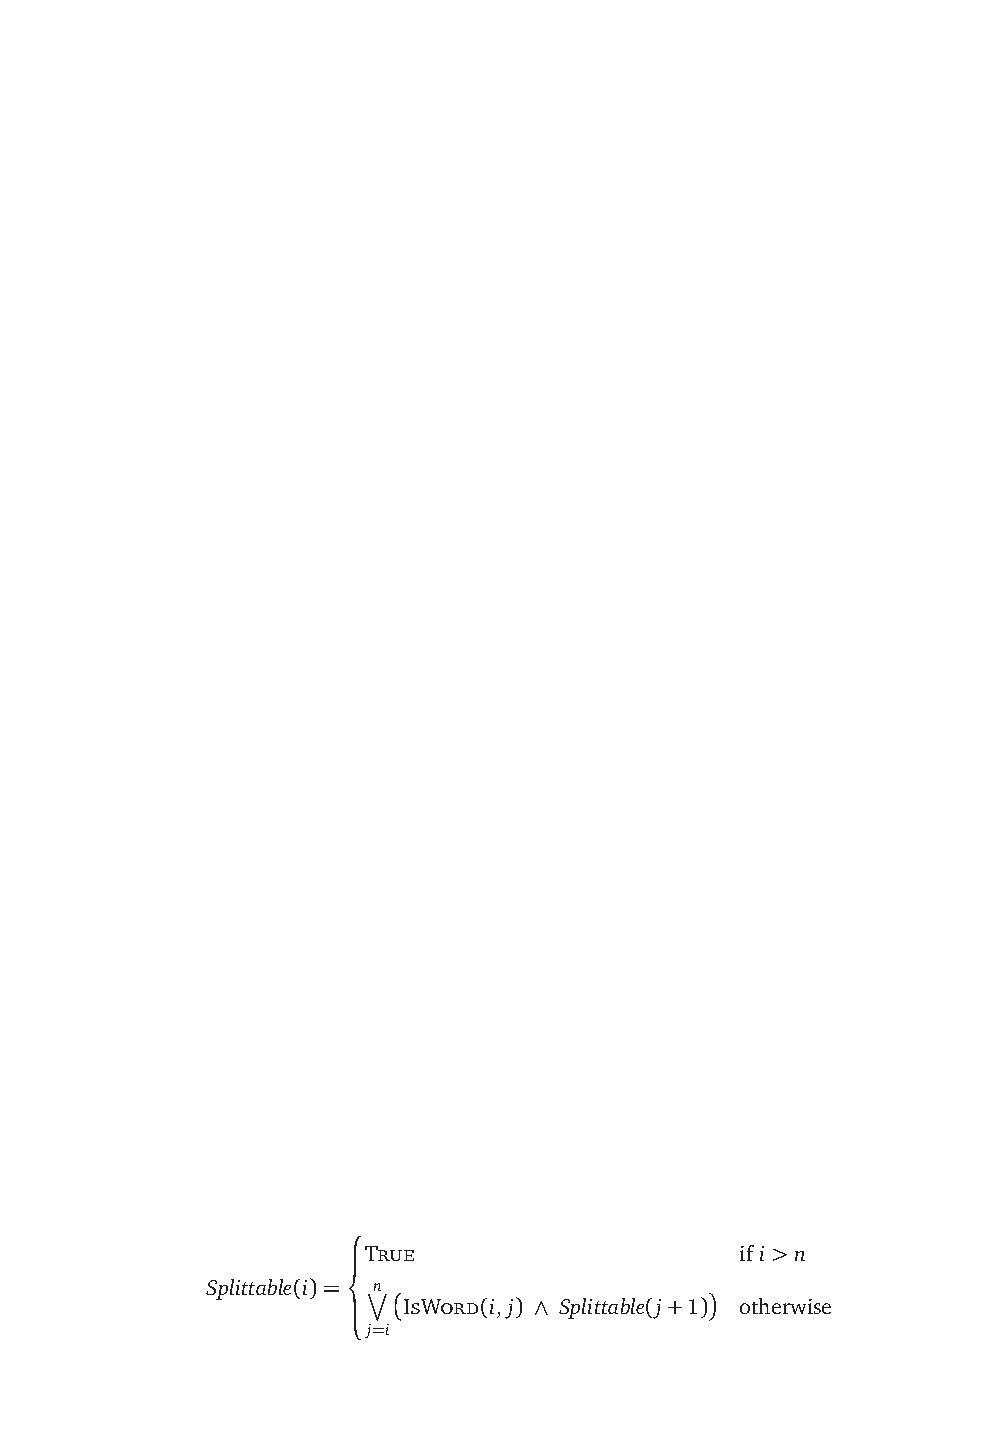
\includegraphics{w05-splittable.pdf}
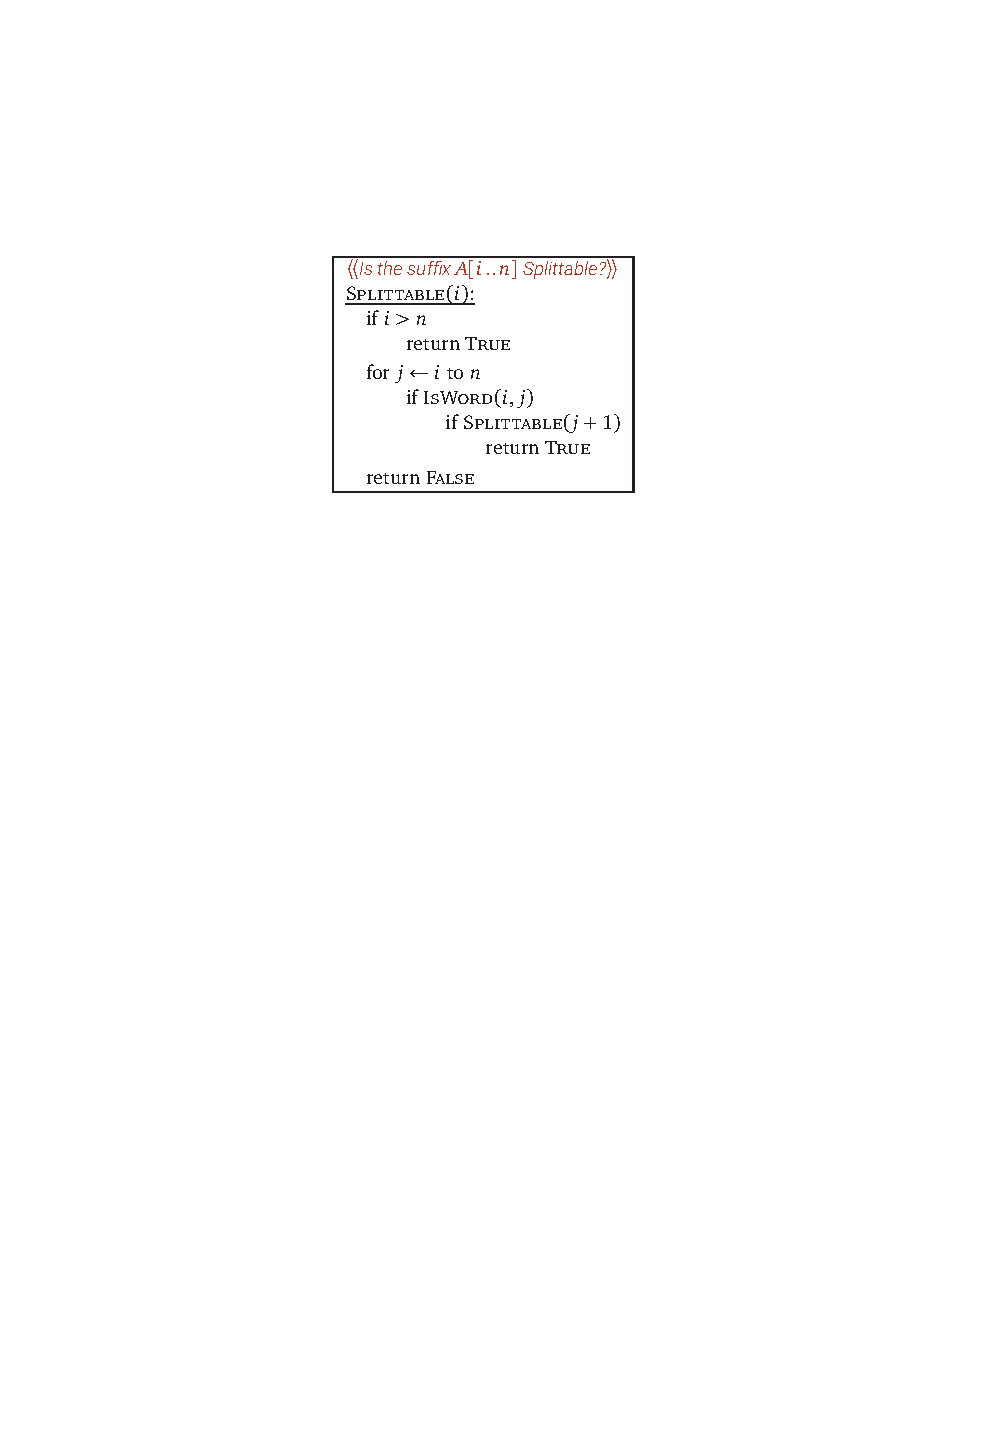
\includegraphics{w05-splittable-pc.pdf}

\vspace{2em}
Pick $i = 5$ (as an example). Which cells of the array $S[0..14]$ does $S[5]$ depend on?
\vspace{2em}

\begin{minipage}{1.0\textwidth}\centering
    \begin{tabular}{lllllllllllllll}
    \hline
    \multicolumn{1}{|l|}{} & \multicolumn{1}{l|}{} & \multicolumn{1}{l|}{} & \multicolumn{1}{l|}{} & \multicolumn{1}{l|}{} & \multicolumn{1}{l|}{} & \multicolumn{1}{l|}{} & \multicolumn{1}{l|}{} & \multicolumn{1}{l|}{} & \multicolumn{1}{l|}{} & \multicolumn{1}{l|}{} & \multicolumn{1}{l|}{} & \multicolumn{1}{l|}{} & \multicolumn{1}{l|}{} & \multicolumn{1}{l|}{} \\ \hline
    0                      & 1                     & 2                     & 3                     & 4                     & 5                     & 6                     & 7                     & 8                     & 9                     & 10                    & 11                    & 12                    & 13                    & 14                   
    \end{tabular}
\end{minipage}%

\begin{itemize}
    \item Write a dynamic programming implementation of \textsc{Splittable}.
\end{itemize}

\vfill

Review Section 3.4 (page 105) in the textbook. 




\end{document}


